% !TeX program = pdflatex
% !TeX spellcheck = en_US
% !TeX encoding = UTF-8

% update
% v.1.2 - 2018-10-15
% - Felix: use Bibtex instead of Biblatex
% v1.10 - 2017-05-30
% - Erik: Refactor the file structure of the front pages
% - Erik: Fix double bibliography entry
% v1.9 - 2017-02-03
% - Dirk: fixed warning: Underfull \hbox (badness 10000) in paragraph main.tex
% - Dirk: fixed warning: "Data encoding is UTF8" -> style.tex 0.1.8
% v1.8 - 2017-02-02
% - Dirk: replaced titlesec package by KOMA-script commands.-> style.tex v0.1.7
% v1.7 - 2014-11-18
% - bib fixes: now using biber instead of bibtex (thanks felix)
% - compile now with pdflatex -> biber -> pdflatex
% v1.6 - 2013-05-13
% - bibliography headers fixed - thanx lorenz lehmann
% - high quality titlepage - thanx thomas graf
% - removed separation of online and offline references -> style 1.4a
% v1.5 - 2013-01-16

\documentclass[twoside,11pt,titlepage,a4paper,english,bibliography=totocnumbered,listof=numbered]{scrbook}
%
% Template Style
% =========================================================================
% = SNET THESIS TEMPLATE STYLE
% =========================================================================

% http://www.snet.tu-berlin.de
% ------------------------
% Adapted version from http://hci.rwth-aachen.de/karrer_thesistemplate (Thorsten Karrer)
% Further adaptions for http://www.elearn.rwth-aachen.de (Sascha Hoellger)
% Further adaptions for SNET @ TU Berlin by Sebastian Göndör (sebastian.goendoer@tu-berlin.de)


% =========================================================================
% = CHANGELOG
% =========================================================================
% [0.1.9]
% - Fixed styling for chapters and toc using Komascript
% - Remove double bibliography TOC entry
%
% [0.1.8]
% - fixed "warning UFT8 is used". biblatex requires ascii encoding; by Dirk
%
% [0.1.7]
% replaced "Titelsec" commands (and whole package) by appropriate KOMA-Script commands; by Dirk
%
% [0.1.6]
% replaced deprecated \rm commands with \rmfamily commands; by Dirk
%
% [0.1.4b]
% backend=biber added in line 139
%
% [0.1.4a]
% title page: image logo sizes and margins adjusted to printable area
% removed separation of online and offline references
%
% [0.1.3]
% wider text body
% added "school" to the titlepage
% paragraph indents
% correctly placed footnote graphics
%
% [0.1.2]
% new titlepage
% some minor fixes
%
% [0.1.1]
% changed titlepage logo
% added listoffigures and listoftables
% excluded abstract from toc
% no (roman) numbering for frontmatter
%
% [0.1]
% adapted version 0.991b from sascha hoellger @ rwth aachen


% =========================================================================
% = MISC
% =========================================================================

\usepackage{a4wide}					%
\usepackage{verbatim}				%
\usepackage[toc,page]{appendix}			%
\usepackage[withpage]{acronym}			%
\usepackage{amsthm}				% Definitions


% =========================================================================
% = COLORS
% =========================================================================

\usepackage{xcolor}					% Colors
\definecolor{LightBlue}{rgb}{0.55,0.55,1}
\definecolor{DarkBlue}{rgb}{0.2,0.2,0.5}
\definecolor{DarkRed}{rgb}{0.71,0.12,0.07}

% =========================================================================
% = PAGE LAYOUT
% =========================================================================

\usepackage{geometry}
\geometry{inner=3cm, outer=2cm, bottom=4cm}

\newcommand{\setwidesite}				% changes the geometry to have less margin
{
	\fancyhfoffset[LE,RO]{0cm}
	\fancyheadoffset[LO,RE]{0cm}
	\fancyfootoffset[RE]{2cm}
	\newgeometry{inner=2cm, outer=2cm, bottom=4cm}
}

\usepackage{style/noindent}				%do not indent at new paragraphs but add a vertical offset

\setlength{\parindent}{4mm}
\setlength{\parskip}{1.5mm }


% =========================================================================
% = TYPESETTING
% =========================================================================

\usepackage[hyphens]{url}				% url
\usepackage{hyphenat}				% hyphenation. use \hyphenation{}

\righthyphenmin=5
\lefthyphenmin=5


% =========================================================================
% = TABLE OF CONTENTS
% =========================================================================

\setcounter{secnumdepth}{4}
\setcounter{tocdepth}{3}

\addtokomafont{disposition}{\rmfamily}


% =========================================================================
% = FONTS
% =========================================================================

\usepackage{mathpazo}
\usepackage[scaled=.95]{helvet}
\usepackage{courier}


% =========================================================================
% = SYMBOLS
% =========================================================================

%\usepackage{gensymb}
\usepackage{textcomp} 				% for \textmu (non-italic $\mu$)
\makeatletter						% this makes "@" a regular letter


% =========================================================================
% = TABLES
% =========================================================================

\usepackage{tabularx}
\usepackage{booktabs}
\usepackage{multirow}
\usepackage{longtable}				% tables spanning over more than one page

%%\setlength{\fboxsep}{0mm}			% spacing between \fbox border and content

\usepackage{amsmath}				% math fonts
\usepackage{amssymb}				% math symbols
\usepackage{setspace}				% line spacing


% =========================================================================
% = BIBILOGRAPHY
% =========================================================================

% 2018-10-16 - changed to use Bibtex instead

%\usepackage[style=numeric,natbib=true,backend=biber]{biblatex}

% apparently no effect?
%\renewcommand{\bibsetup}{
%	\markboth{
%		\MakeUppercase{Bibliography}
%	}{}
%}

%\ifdefined\bibheadingonline
%  \defbibheading{online}{\section*{\bibheadingonline}}
%\else
%  \defbibheading{online}{\section*{Online References}}
%\fi
%\ifdefined\bibheadingoffline
%  \defbibheading{offline}{\section*{\bibheadingoffline}}
%\else
%  \defbibheading{offline}{\section*{Printed References}}
%\fi
%
%\defbibfilter{online}{%
%  \( \type{online} \)}
%
%\defbibfilter{offline}{%
%  \( \not \type{online} \)}
%
%\bibliography{Bibliography}


% =========================================================================
% = LANGUAGE & ENCODING
% =========================================================================

\usepackage[english]{babel}				% \usepackage[ngerman]{babel}

\selectlanguage{english}				% \selectlanguage{ngerman}

\usepackage[T1]{fontenc}
\usepackage[utf8]{inputenc}				% can use native umlauts

% \usepackage[babel,german=quotes]{csquotes}	% provides \enquote{Blupp} => "`Blupp"'
\usepackage[babel,english=american]{csquotes}	% provides \enquote{Blupp} => "`Blupp"'

%\SetCiteCommand{\parencite}			% Changed for biblatex

\usepackage{units}					% unified way of setting values with units

\usepackage{appendix}


% =========================================================================
% = CODE LISTINGS
% =========================================================================

\usepackage{listings}

% Listings Styles from Max

\definecolor{violet}{cmyk}{0.45,0.97,0.27,0.21}
\definecolor{lstblue}{cmyk}{1,0.80,0,0}
\definecolor{lstgreen}{cmyk}{0.71,0.21,0.65,0.22}
\definecolor{bluegrey}{cmyk}{0.56,0.24,0.11,0.05}
\definecolor{javadoc}{cmyk}{0.88,0.59,0,0}
\definecolor{lstgrey}{cmyk}{0.55,0.44,0.42,0.32}

\lstdefinelanguage{SQL}{
     keywords={},
     keywordstyle=\color{bluegrey}\bfseries,
     morekeywords=[2]{CREATE,TABLE,IF,NOT,EXISTS,NULL,SET,DEFAULT,PRIMARY,KEY,COLLATE,CHARACTER,AUTO_INCREMENT,ENGINE,CHARSET},
     keywordstyle={[2]\color{violet}\bfseries},
     otherkeywords={int,varchar,double,text,tinyint},
     sensitive=false,
     morecomment=[l][\color{lstgreen}]{//},
     morecomment=[s][\color{lstgreen}]{/*}{*/},
     morecomment=[s][\color{javadoc}]{/**}{*/},
     morestring=[b]',
     morestring=[b]"
  }
\lstdefinelanguage{PHP}{
     keywords={},
     keywordstyle=\color{bluegrey}\bfseries,
     morekeywords=[2]{static,function,if,return,pow,sin,cos,asin,min,sqrt,int},
     keywordstyle={[2]\color{violet}\bfseries},
     otherkeywords={@param, @returns, @author, @type, @link, @see},
     sensitive=false,
     morecomment=[l][\color{lstgreen}]{//},
     morecomment=[s][\color{lstgreen}]{/*}{*/},
     morecomment=[s][\color{javadoc}]{/**}{*/},
     morestring=[b]',
     morestring=[b]"
  }
\lstdefinelanguage{JavaScript}{
     keywords={},
     keywordstyle=\color{bluegrey}\bfseries,
     morekeywords=[2]{attributes, class, classend, do, empty, endif, endwhile, fail, function, functionend, if, implements, in, inherit, inout, not, of, operations, out, return, set, then, types, while, use},
     keywordstyle={[2]\color{violet}\bfseries},
     otherkeywords={@param, @returns, @author, @type, @link, @see},
     sensitive=false,
     morecomment=[l][\color{lstgreen}]{//},
     morecomment=[s][\color{lstgreen}]{/*}{*/},
     morecomment=[s][\color{javadoc}]{/**}{*/},
     morestring=[b]',
     morestring=[b]"
  }
\lstdefinelanguage{Java}{
     keywords={},
     keywordstyle=\color{bluegrey}\bfseries,
     morekeywords=[2]{abstract,boolean,break,byte,case,catch,char,class,
      const,continue,default,do,double,else,extends,false,final,
      finally,float,for,goto,if,implements,import,instanceof,int,
      interface,label,long,native,new,null,package,private,protected,
      public,return,short,static,super,switch,synchronized,this,throw,
      throws,transient,true,try,void,volatile,while},
     keywordstyle={[2]\color{violet}\bfseries},
     morekeywords=[3]{@SuppressWarnings, @Capability, @Override},
     keywordstyle={[3]\color{lstgrey}},
     otherkeywords={@param, @return, @returns, @author, @link, @see},
     sensitive,
     morecomment=[l]//,
     morecomment=[s]{/*}{*/},
     morecomment=[s][\color{javadoc}]{/**}{*/},
     morestring=[b]",
     morestring=[b]',
  }[keywords,comments,strings]

% some listings styles from Gregor Aisch
% http://vis4.net/blog/2009/09/noch-mehr-sprach-definitionen-fuer-latex-listings/

\lstdefinelanguage{HTML5} {morekeywords={a, abbr, address, area, article, aside, audio, b, base, bb, bdo, blockquote,  body, br, button, canvas, caption, cite, code, col, colgroup, command, datagrid, datalist, dd, del, details, dialog, dfn, div, dl, dt, em, embed, eventsource, fieldset, figure, footer,  form,  h1, h2,  h3,  h4, h5,  h6,  head,  header,  hr, html,  i, iframe,  img,  input,  ins, kbd,  label,  legend,  li,  link,  mark,  map,  menu,  meta,  meter,  nav,  noscript,  object,  ol,  optgroup,  option,  output,  p,  param,  pre,  progress,  q,  ruby,  rp,  rt,  samp,  script,  section,  select,  small,  source,  span,  strong,  style,  sub,  sup,  table,  tbody,  td,  textarea,  tfoot,  th,  thead,  time,  title,  tr,  ul,  var,  video},
sensitive=false, morecomment=[s]{<!--}{-->}, morestring=[b]", morestring=[d]'}

\lstdefinelanguage{CSS} {morekeywords={azimuth,  background-attachment,  background-color,  background-image,  background-position,  background-repeat,  background,  border-collapse,  border-color,  border-spacing,  border-style,  border-top, border-right, border-bottom, border-left,  border-top-color, border-right-color, border-bottom-color, border-left-color,  border-top-style, border-right-style, border-bottom-style, border-left-style,  border-top-width, border-right-width, border-bottom-width, border-left-width,  border-width,  border,  bottom,  caption-side,  clear,  clip,  color,  content,  counter-increment,  counter-reset,  cue-after,  cue-before,  cue,  cursor,  direction,  display,  elevation,  empty-cells,  float,  font-family,  font-size,  font-style,  font-variant,  font-weight,  font,  height,  left,  letter-spacing,  line-height,  list-style-image,  list-style-position,  list-style-type,  list-style,  margin-right, margin-left,  margin-top, margin-bottom,  margin,  max-height,  max-width,  min-height,  min-width,  orphans,  outline-color,  outline-style,  outline-width,  outline,  overflow,  padding-top, padding-right, padding-bottom, padding-left,  padding,  page-break-after,  page-break-before,  page-break-inside,  pause-after,  pause-before,  pause,  pitch-range,  pitch,  play-during,  position,  quotes,  richness,  right,  speak-header,  speak-numeral,  speak-punctuation,  speak,  speech-rate,  stress,  table-layout,  text-align,  text-decoration,  text-indent,  text-transform,  top,  unicode-bidi,  vertical-align,  visibility,  voice-family,  volume,  white-space,  widows,  width,  word-spacing,  z-index},
sensitive=false, morecomment=[s]{/*}{*/}, morestring=[b]", morestring=[d]'}

\lstdefinelanguage{JavaFX} {morekeywords={abstract, after, and, as, assert, at, attribute, before, bind, bound, break, catch, class, continue, def, delete, else, exclusive, extends, false, finally, first, for, from, function, if, import, indexof, in, init, insert, instanceof, into, inverse, last, lazy, mixin, mod, new, not, null, on, or, override, package, postinit, private, protected, public-init, public, public-read, replace, return, reverse, sizeof, static, step, super, then, this, throw, trigger, true, try, tween, typeof, var, where, while, with },
sensitive=false, morecomment=[l]{//}, morecomment=[s]{/*}{*/}, morestring=[b]", morestring=[d]'}

\lstdefinelanguage{MXML} {morekeywords={mx:Accordion, mx:Box, mx:Canvas, mx:ControlBar, mx:DividedBox, mx:Form, mx:FormHeading, mx:FormItem, mx:Grid, mx:GridItem, mx:GridRow, mx:HBox, mx:HDividedBox, mx:LinkBar, mx:Panel, mx:TabBar, mx:TabNavigator, mx:Tile, mx:TitleWindow, mx:VBox, mx:VDividedBox, mx:ViewStack, mx:Button, mx:CheckBox, mx:ComboBase, mx:ComboBox, mx:DataGrid, mx:DateChooser, mx:DateField, mx:HRule, mx:Image, mx:Label, mx:Link, mx:List, mx:Loader, mx:MediaController, mx:MediaDisplay, mx:MediaPlayback, mx:MenuBar, mx:NumericStepper, mx:ProgressBar, mx:RadioButton, mx:RadioButtonGroup, mx:Spacer, mx:Text, mx:TextArea, mx:TextInput, mx:Tree, mx:VRule, mx:VScrollBar, mx:Application, mx:Repeater, mx:UIComponent, mx:UIObject, mx:View, mx:FlexExtension, mx:UIComponentExtension, mx:UIObjectExtension, mx:Fade, mx:Move, mx:Parallel, mx:Pause, mx:Resize, mx:Sequence, mx:WipeDown, mx:WipeLeft, mx:WipeRight, mx:WipeUp, mx:Zoom, mx:EventDispatcher, mx:LowLevelEvents, mx:UIEventDispatcher, mx:CurrencyFormatter, mx:DateFormatter, mx:NumberFormatter, mx:PhoneFormatter, mx:ZipCodeFormatter, mx:CursorManager, mx:DepthManager, mx:DragManager, mx:FocusManager, mx:HistoryManager, mx:LayoutManager, mx:OverlappedWindows, mx:PopUpManager, mx:SystemManager, mx:TooltipManager, mx:CreditCardValidator, mx:DateValidator, mx:EmailValidator, mx:NumberValidator, mx:PhoneNumberValidator, mx:SocialSecurityValidator, mx:StringValidator, mx:ZipCodeValidator, mx:DownloadProgressBar, mx:ArrayUtil, mx:ClassUtil, mx:Delegate, mx:ObjectCopy, mx:URLUtil, mx:XMLUtil, mx:CSSSetStyle, mx:CSSStyleDeclaration, mx:CSSTextStyles, mx:StyleManager, mx:HTTPService, mx:RemoteObject, mx:Service},
sensitive=false, morecomment=[s]{<!--}{-->}, morestring=[b]", morestring=[d]'}

\lstdefinelanguage{LZX} {morekeywords={a, alert, animator, animatorgroup , attribute, audio , axis, axisstyle , b, barchart, basebutton , basebuttonrepeater , basecombobox , basecomponent , basedatacombobox , basedatepicker , basedatepickerday , basedatepickerweek , basefloatinglist , basefocusview , baseform , baseformitem , basegrid , basegridcolumn , baselist , baselistitem , basescrollarrow , basescrollbar , basescrollthumb , basescrolltrack , baseslider , basestyle , basetab , basetabelement , basetabpane , basetabs , basetabsbar , basetabscontent , basetabslider , basetrackgroup , basetree , basevaluecomponent , basewindow , br , button , canvas , chart , chartbgstyle , chartstyle , checkbox , class , columnchart , combobox , command , connection , connectiondatasource , constantboundslayout , constantlayout , datacolumn , datacombobox , datalabel , datamarker , datapath , datapointer , dataselectionmanager , dataseries , dataset , datasource , datastyle , datastylelist , datatip , datepicker , debug , dragstate , drawview , edittext , event , face , floatinglist , font , font , form , frame , grid , gridcolumn , gridtext , handler , hbox , horizontalaxis , hscrollbar , i , image , img , import , include , inputtext , javarpc , label , labelstyle , layout , legend , library , linechart , linestyle , list , listitem , LzTextFormat , menu , menubar , menuitem , menuseparator , method , modaldialog , multistatebutton , node , p , param , piechart , piechartplotarea , plainfloatinglist , plotstyle , pointstyle , pre , radiobutton , radiogroup , rectangularchart , regionstyle , remotecall , resizelayout , resizestate , resource , reverselayout , richinputtext , rpc , script , scrollbar , security , selectionmanager , sessionrpc , simpleboundslayout , simpleinputtext , simplelayout , slider , soap , splash , stableborderlayout , state , statictext , style , submit , swatchview , SyncTester , tab , tabelement , tabpane , tabs , tabsbar , tabscontent , tabslider , Test , TestCase , TestResult , TestSuite , text , textlistitem , tickstyle , tree , u , valueline , valuelinestyle , valuepoints , valuepointstyle , valueregion , valueregionstyle , vbox , verticalaxis , view , view , vscrollbar , webapprpc , window , windowpanel , wrappinglayout , XMLHttpRequest , xmlrpc , zoomarea},
sensitive=false, morecomment=[s]{<!--}{-->}, morestring=[b]", morestring=[d]'}

\lstset{
  numbers=left,
  numberstyle=\tiny,
  numbersep=5pt,
  breaklines=true,
  stepnumber=1,
  tabsize=2,
  basicstyle=\ttfamily\small,
  frame=none,
  numberfirstline=true,
  firstnumber=1,
  keywordstyle=\color{violet}\bfseries,
  ndkeywordstyle=\color{bluegrey}\bfseries,
  identifierstyle=\color{black},
  commentstyle=\color{lstgreen}\ttfamily,
  stringstyle=\color{lstblue}\ttfamily,
  showstringspaces=false
}


% ========================================================================
% = CHANGE LIST DEFINITIONS
% ========================================================================

% change color of item list
\renewcommand{\labelitemi}{\color{DarkRed}$\bullet$}
\renewcommand{\labelitemii}{\color{DarkRed}$\circ$}
\renewcommand{\labelitemiii}{\color{DarkRed}$\ast$}
\renewcommand{\labelitemiv}{\color{DarkRed}$\diamond$}

% change color of enum list
\renewcommand{\labelenumi}{\color{DarkRed}\arabic{enumi}.}
\renewcommand{\labelenumii}{\color{DarkRed}\alph{enumii})}
\renewcommand{\labelenumiii}{\color{DarkRed}\roman{enumiii}.}
\renewcommand{\labelenumiv}{\color{DarkRed}\Alph{enumiv}.}

% change color of description list
\usepackage{enumitem}
\setdescription{font=\color{DarkRed}\rmfamily\itshape}
% \renewenvironment{description}{\list{font=\color{DarkRed}\itshape}}{\endlist}


% ========================================================================
% = FOOTNOTES
% ========================================================================

% change color of footnotes
\renewcommand{\thefootnote}{\color{DarkRed}\arabic{footnote}}

% use nice footnote indentation
\deffootnote[1em]{1em}{1em}{\textsuperscript{\thefootnotemark}\,}


% =========================================================================
% = GRAPHICS AND IMAGES
% =========================================================================

\usepackage{graphicx}
\graphicspath{{images/}}				% path to your image folder

\usepackage{eso-pic}					% needed for the full-face titlepage
\usepackage{chngpage}				% we need this to determine if a figure is on an odd or even page
\usepackage{tikz}					% tikz pictures

% captions of tables and images
\usepackage[hang,small,sf]{caption}
\renewcommand{\captionfont}{\sffamily\small}
\renewcommand{\captionlabelfont}{\bfseries}

\usepackage{float}
\usepackage{placeins}
% \floatstyle{ruled}
%\floatplacement

\renewcommand{\floatpagefraction}{0.85}		% if a figure takes more than 85% of a page it will be typeset on a separate page
\usepackage[it,bf,tight,hang,raggedright]{subfigure}

%\numberwithin{figure}{section}
%\numberwithin{table}{section}


% =========================================================================
% = HEADER
% =========================================================================

\newcommand{\STYLEfootnotetext}
{
  \begin{minipage}
  {.2\textwidth}
    
\includegraphics[width=0.9\textwidth]{images/snet/snet_footer.png}
  \end{minipage}
}

% Change page headers and footers:
\usepackage{calc}
\usepackage{fancyhdr}
\pagestyle{fancy}
\fancyhfoffset[RO,LE]{0.1cm} %{\marginparsep+\marginparwidth}
\fancyhfoffset[RE,LO]{0.1cm}
%\fancyheadoffset[RE,LO]{\hoffset + \oddsidemargin}
\renewcommand{\headrule}{{\color{DarkRed}%
  \hrule width\headwidth height\headrulewidth \vskip-\headrulewidth}}
\fancyhf{}
\fancyhead[RE]{\slshape \nouppercase{\leftmark}}    % Even page header: "page   chapter"
\fancyhead[LO]{\slshape \nouppercase{\rightmark}}   % Odd  page header: "section   page"
\fancyhead[RO,LE]{\bfseries \thepage}

%- \fancyfoot[LE]{\STYLEleftpicture}
%- \fancyfoot[RO]{\STYLErightpicture}
\fancyfoot[LE]{\STYLEfootnotetext}

\renewcommand{\headrulewidth}{1pt}    % Underline headers
\renewcommand{\footrulewidth}{0pt}

% =========================================================================
% = SECTIONS THEMING
% =========================================================================

\newcommand{\allsectionformat}{\color{DarkRed}\rmfamily\normalfont}

% Font style and colors
\addtokomafont{part}{\Huge\allsectionformat}
\addtokomafont{chapter}{\Huge\allsectionformat}
\addtokomafont{section}{\allsectionformat}
\addtokomafont{subsection}{\allsectionformat}
\addtokomafont{subsubsection}{\allsectionformat}
\addtokomafont{paragraph}{\allsectionformat}
\addtokomafont{subparagraph}{\allsectionformat}

% Spacing before and after the section titles
\RedeclareSectionCommand[
  beforeskip=-.75\baselineskip,
  afterskip=.5\baselineskip]{section}

\RedeclareSectionCommand[
  beforeskip=-5\baselineskip,
  afterskip=.5\baselineskip]{chapter}


% =========================================================================
% = TYPESETTING - TWEAKES
% =========================================================================

\addtokomafont{section}{\LARGE}
\addtokomafont{subsection}{\large}

% instead of sloppy
%\tolerance 1414
%\hbadness 1414
%- \tolerance 2414
%- \hbadness 2414
%- \emergencystretch 1.5em
%- \hfuzz 0.3pt
%- \widowpenalty=10000     % Hurenkinde r
%- \clubpenalty=10000      % Schusterjungen
%- \brokenpenalty=10000
%- \interlinepenalty=9000 % seitenumbruch im absatz
%- \vfuzz \hfuzz
%- \raggedbottom


% =========================================================================
% =  USER DEFINED COMMANDS
% =========================================================================

\newcommand{\chapterquote}[2]{
    \begin{quotation}
    \begin{flushright}
    \noindent\emph{``{#1}''\\[1.5ex]---{#2}}
    \end{flushright}
    \end{quotation}
}


% custom hyphenation					% add words to this list to prevent hyphenation
\hyphenation{
ASCII
TCP
}

%make readable references
\usepackage[pdftex,pdfpagelabels=true]{hyperref}
\hypersetup{%
	pdftitle={Thesis Title},
	pdfauthor={Thesis Author},
	pdfkeywords={key1, key2, key3},
	pdfsubject={Thesis Subject}
}

% Adding a finite stretch on the page suppresses "Underfull \vbox (badness 10000)" warnings.
\makeatletter
\def\@textbottom{\vskip \z@ \@plus 1pt}
\let\@texttop\relax
\makeatother

\begin{document}

%--------------------------------------------------------------
% FRONT PAGE AND DOCUMENT METADATA
%--------------------------------------------------------------
\frontmatter

\begin{titlepage}
	\AddToShipoutPicture*{
		\put(0,0){
			
\includegraphics[width=\paperwidth,height=\paperheight,keepaspectratio=false]{images/snet/titlepage.pdf}
		}
	}
	\strut
	\hfill
	\begin{center}
	\vspace{1cm}
		\Huge
		\begin{spacing}{.9}
			\textcolor{DarkRed}{\textbf{A solar powered flux capacitor}}\\
		\end{spacing}
		\vspace{0.8cm}
		\large
		by\\
		\vspace{0.8cm}
		\textbf{Emmet Brown}\\
		\vspace{0.8cm}
		\textbf{Matriculation Number 123456}\\
		\vspace{2cm}
	 	A thesis submitted to\\
		\vspace{0.5cm}
		Technische Universität Berlin\\
		School IV - Electrical Engineering and Computer Science\\
		Department of Telecommunication Systems\\
		Service-centric Networking\\
		\vspace{0.5cm}
		Master's Thesis\\
		\vspace{2.2cm}
		\today\\
		\vspace{2.0cm}
		\large
		Supervised by:\\
		Prof. Dr. Axel Küpper\\
		\vspace{1cm}
		Assistant supervisor:\\
		Dr. Dr. Chuck Norris
		\end{center}
         		%
\includegraphics[scale=1.0]{images/watermark.png}
\end{titlepage}

% Clear two pages after the title
\shipout\null
\shipout\null

\chapter*{\LARGE Eidestattliche Erklärung / Statutory Declaration}
Hiermit erkläre ich, dass ich die vorliegende Arbeit selbstständig und eigenhändig sowie ohne unerlaubte fremde Hilfe und ausschließlich unter Verwendung der aufgeführten Quellen und Hilfsmittel angefertigt habe.
\vspace{2em}

\noindent I hereby declare that I have created this work completely on my own and used no other sources or tools than the ones listed.

\vspace{30 mm}
\begin{flushright}

\rule{90mm}{1pt}

Berlin, \today \hspace{15 mm} Chuck Norris' son
\end{flushright}

%\chapter*{Acknowledgement}
\label{cha:acknowledgments}
\vspace{20 mm}

 It was a remarkable experience to work as a team with these incredibly skilled members especially Mohammed Haseeb Asif, who single-handedly overlooked the entire development phase serving as a highly capable Project Manager with his years of impeccable experience on Software Industry.

We would like to express our deepest appreciation to all those who have helped us to successfully complete this project. A special gratitude to our supervisor Mr.Marcel Müller, whose contribution in terms of guidance, advice and helping us to keep motivated throughout the project. 


We would like to thank the SNET faculty for providing us this opportunity to work on the project with a set of enthusiastic team members and a great mentor. We would also like to thank all other mentors, friends, motivators, critiques, supporters and well-wishers who have helped us finalizing this project within the limited time frame. 

\vspace{20 mm}
\noindent Thanks, 
\vspace{2 mm}

\noindent Group 6



\chapter*{Abstract}
\label{cha:abstract}

The purpose of this documentation is to present our project. The project requirement was to develop a Dashboard web parcel management service. We established an interface system that could be used by courier-companies\textbackslash customers\textbackslash postman's for monitoring and updating the package status and condition. The package data is being store in the blockchain, therefore the data is cross-company own. For bringing the data from the blockchian to the dashboard we developed a backend communication level API.
The system enable all parties involve in the package delivery to communicate with one uncentrelized source.					% EN Abstract
\chapter*{Zusammenfassung}
\label{cha:zusammenfassung}

Hier kommt das deutsche Abstract hin. Wie das geht, kann man wie immer auf Wikipedia nachlesen \url{http://de.wikipedia.org/wiki/Abstract}...	% DE Abstract

\tableofcontents{}

%--------------------------------------------------------------
% MAIN CONTENT
%--------------------------------------------------------------
\mainmatter

%\part{}						% optional: use parts to structure your thesis
\chapter{Introduction}
\label{cha:introduction}

% \chapterquote{I'm awesome!}{Barney Stinson, WIRED magazine, 19.1.2009}

\section{Background}

As companies and consumers increasingly purchase goods online, the demand for cross carrier management platform
delivery services grows (First Research 2013, 7). Furthermore, the growth of online retail
sales has influenced the logistics industry for the past ten years and the trend is expected to
continue at least on a similar level during the next few years. (Delfmann et al. 2002, 203.) 

\begin{figure}[!ht]
	\centering
	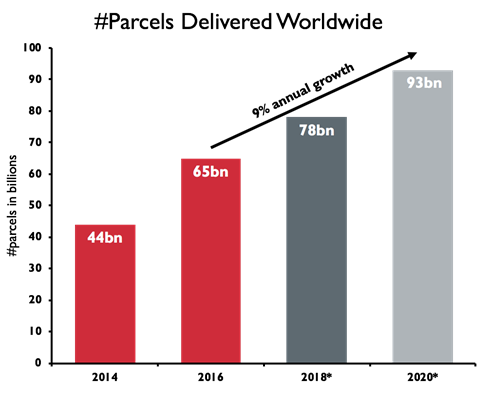
\includegraphics[width=0.5\textwidth]{images/ParcelsDel.png}\\
	\caption{Parcels Delivered worldwide [billions]}
	\label{fig:introduction__loremipsum}
\end{figure}

Responding to the increased demand of small-sized frequent shipments incurred by e-commerce has become one of the biggest challenges for logistics express delivery companies.
A successful delivery of shipments to consumers distributed across large geographical areas
will require re-designing of the existing system.

The increase of business-to-consumer (B2C) e-commerce activities implies that business are border less, global e-commerce is selling products or offer services across the world.


The idea to investigate delivery service based on the  blockchain proposed by the TU Berlin. The DC3 team in this project did not focus on implementing the blockchain system but rather in creating a platform interface to manage the parcel. At the end of the day, DC3 aims to be a part of a B2B blockchain solution that will make cross-border logistics much more reliable and efficient than they are now.   

Parcels are not always delivered at their destination in time and with the right agreed quality, this can cause financial losses due to reimbursements and low customer satisfaction. Especially higher value shipments ranging from routine parcels up to extraordinary parcels are insured against risks of loss, theft, damage or any other events that could impact delivery precision and quality. Prompt and secure detection, monitoring and recording of the shipment events is needed to allow tracking of service quality level, accountability, liability evidence in disputes and for analysis and optimization of the logistical chain.

DC3 (Dashboard for Control and Communication center) is a web-based dashboard for monitoring and controlling the logistics transactions beyond the border of a certain logistics company while leveraging DiLLaS (distributed ledger for logistics and supply chain management (DiLLaS). 

DiLLaS is an IoT and Blockchain solution that offers a new and unique view on shipment events data for logistics companies and their partners. These views create a detailed insight and transparency of significant security and safety events during the shipment. Additionally, by storing them in the distributed ledger, a trusted and decentralized recollection of the events of the shipment is created. DC3 enables a new way of handling parcel delivery and accelerates the implementation of more reliable and financial sustainable delivery processes.

The goal of DiLLaS is to provide a distributed ledger for the secure and trustworthy storage of events that occur during the transport of goods. A DiLLaS Mobile App will act as a client for the ledger and is intended as a means for all participants of a logistic chain to securely log a registration, deregistration and handover of a parcel within the distributed ledger. In combination with GRAVITY, the DiLLaS Mobile App will in addition be able to check the status of sensors that are attached to the parcels such temperature or humidity sensors and to log violations of predefined delivery conditions within the distributed ledger. Since DiLLaS makes use of Blockchain technology to persist the events and their related data in an immutable, transparent and a distributed manner where common incidents such as lost or delayed parcels can be securely traced back to its originators. With the commonly approved log of logistic events in DiLLaS, logistic operators will be able to improve their efficiency in terms of parcel delivery time by identifying bottle necks, costs per parcel by identifying unreliable partners and the quality of service by evaluating if parcels are delivered according to the predefined delivery conditions such as a constant temperature or an acceptable intensity of shocks for goods of high value. 


\section{Problem Discussion}

\subsection{Vendors communication and limitations}
There are multiple inefficiencies in cross-border delivery industry, related to lack of transparency and trust between the different logistics providers. International parcel delivery usually go through several logistics vendor, each on their side of the border, and there is a lot of accounting and interoperability overhead in the interactions between the different vendors. The idea is to solve these issues with the blockchain technology, taking advantage of its inherent transparency and trust.
From a Logistic company perspective, the parcel information is limited to their ownership and post completion of handover to a peer logistic company the package would not be efficiently tracked and the interrelated companies handling the package would not be in consensus. This common interface provides a plausible solution to the problem stated above by giving an opportunity for the companies to keep track of the package irrespective of the ownership of the package at a given point of time by having full information about it. It will also help the companies achieve better customer satisfaction by providing such sensor options to its customers to make use of.

\subsection{Vendors HMI}
From a customer perspective, when a customer orders a parcel the information revealed to him is depended on the quality of the carrier web interface, with a unique high-detailed dashboard the customer can be independent from the retail interface system and be informed about the status of the package and location of the package at all times throughout the journey of the package from source to destination.More options are made available to the customer in terms of a temperature and a shock sensor which is capable of taking lower and upper limits from the customer as an input and reverting with any irregularities in the package.

\chapter{Related Work}
\label{cha:relatedwork}

Historically messages were usually hand-delivered using a variety of methodologies, the most common being runners and horseback riders. Then came the introduction of mechanized courier services which differed from ordinary mail services by features such as speed, security,tracking and individualization of express services. They not only started providing such services within a town or a city but started offering worldwide services. The problem being very evident with such services is tracking these packages as stated above. Such offer services are made worldwide, typically with hub and spoke model. The spoke-hub distribution paradigm is a form of transport topology optimization in which the companies organize routes as a series of "spokes" that connect the outlying points to a central "hub"[1].

These companies further utilize courier software which provide electronic proof of delivery and electronic tracking details of the package limited to ownership. Currently the gap incorporated among logistic companies on cross country deliveries are handled using basic communication or with the help of some third party companies. Eurosender is one such  company that provides a platform for businesses and individuals to have a unified solution to run their logistics processes globally. They provide services for customers ranging from a simple package delivery to Freight transport. They also help their customers track the package based on individual  tracking numbers produced by each of the logistic companies for the delivery of the packages.

Further with respect to look and feel of the application being developed, we were provided with a front-end SPA template "Crystal React Bootstrap Dashboard". Crystal React Bootstrap is a multipurpose admin dashboard created using the technologies React,Redux and Bootstrap. Its main goal is to help create complex applications using a lot of simple and easy to use React components that are embedded in this template. This template is helpful to create many kinds of dashboards relating to the health sector, online social networking websites and also for companies in need of a dashboard.

This template mainly consists of the below mentioned simple packages that could be useful for the development of an end-to-end application.

\begin{itemize}
\item Charts
\item Buttons
\item Notifications
\item Sweet Alert
\item Redux Form
\item AirBnB React Dates
\item Google Map and Uber Vector Map
\item React Bootstrap Table
\item React Big Calendar
\end{itemize}

\chapter{Concept and Design}
\label{cha:conceptanddesign}

DC3 dashboard has 3 different types of personas - Company, Customer and Postman. Hence we had to design the system differently for each user persona. Our front end application is a Single Page Application (SPA) using react JS. Our back-end is developed by using Node JS leveraging Express framework. 

\section{Architecture}
DC3 follows a modular approach for the whole system. As shown in the bigger picture, entry point for the system is social login, Google in this case. we are using passportJS which can be used to integrate other social strategies e.g. GitHub, Facebook as well. Furthermore, passport does provide local strategy as well where we can configure local database as well for authentication and authorization. This feature would be useful when we different vendors does deploy their own instances of the diLLas service and want to authorize the existing customer base from their own system. we have detailed overview for google authorization explained later as well 

\begin{figure}[!ht]
	\centering
	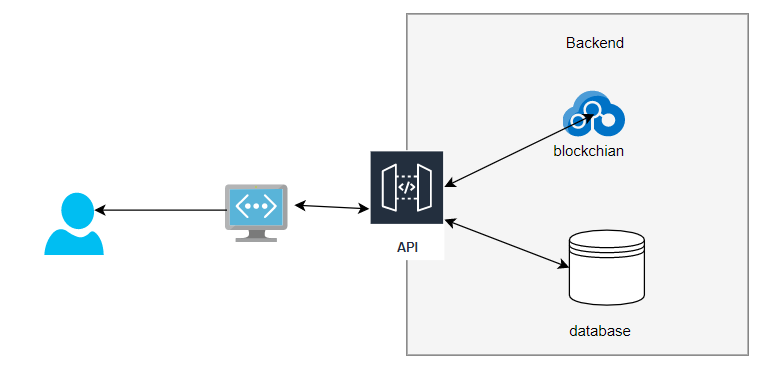
\includegraphics[width=1 \textwidth]{images/bigger_picture.png}\\
	\caption{System Architecture(abstract view)}
	\label{fig:System Architecture(abstract view)}
\end{figure}

Once user is logged-in, for example from browser, an access-token is stored into the local session storage for being used on the front end SPA (Single Page Application) react app.  This token is used for further communication between front-end and back-end. It contains user profile and authorization info. This info is leveraged to protect the different endpoints on the server side and provide related data based on the user type. For example, when a customer hits the /packages endpoint he will be able to see his own packages only but when a company user hits the same endpoint, he will get all the company level packages in the response.

\section{Authentication and Authorization with Google}
Authentication is a vital part of the project and most real world applications need authentication and authorization. While authentication identifies some entity as a valid user, authorization defines the actions that the user is allowed to perform, based on his/her roles and rights. There are many solutions to provide for authentication or authorization in an application and we had two major choices,

\begin{itemize}
\item First one was to keep user state management on Redux.
\item Second was to use a Facebook or a Google Authentication integration with our application.
\end{itemize}

We chose to go with the second choice as it was a new learning for the team to integrate it with our application, reduces the burden for the users to register themselves rather directly sign in with their Google accounts and more importantly because it provides back-end services to securely authenticate users, paired with easy-to-use client SDKs. It can authenticate users using passwords and federated identity provider credentials. 

In our application, once the user clicks on the Google authenticate button,it directs the user to Google's OAuth 2.0 server, which requests access to the user's meta data from the Google drive with a read only scope. Further after granting or denying the access to the user, is then redirected to the original page, which pareses the access token from the string. The page then uses this access token to make  a simple API request which calls the Drive API's to retrieve the information about the authorized user's Google account. If this request is successful then the API response is logged in the browser.
For the first time user's we check our local database to determine the existence and add the user to our database if the user name does not exist and fill in the vital information using the above fetched information from the authorized user's Google account. If the user name exists before hand, we validate the token from the server side with the OAuth2.0 provider and once validated, a JSON Web Token (JWT)  is produced to securely provide authorization to the front end.
We use a main component in our database table "Persons" that is "PersonType" component which determines the role given to a user.Based on this value we determine if the user is either a customer,postman or a company representative. The role with the lowest features is the role of a user, which is the value provided by default to the user on first time log in and henceforth the company role has  authorization to upgrade the user to a postman or a company representative. Initial company role setup is done by the admin. The below figure provides a overview of the functioning of the Google authentication and Authorization based on role integrated to our DC3 application.

\begin{figure}[!ht]
	\centering
	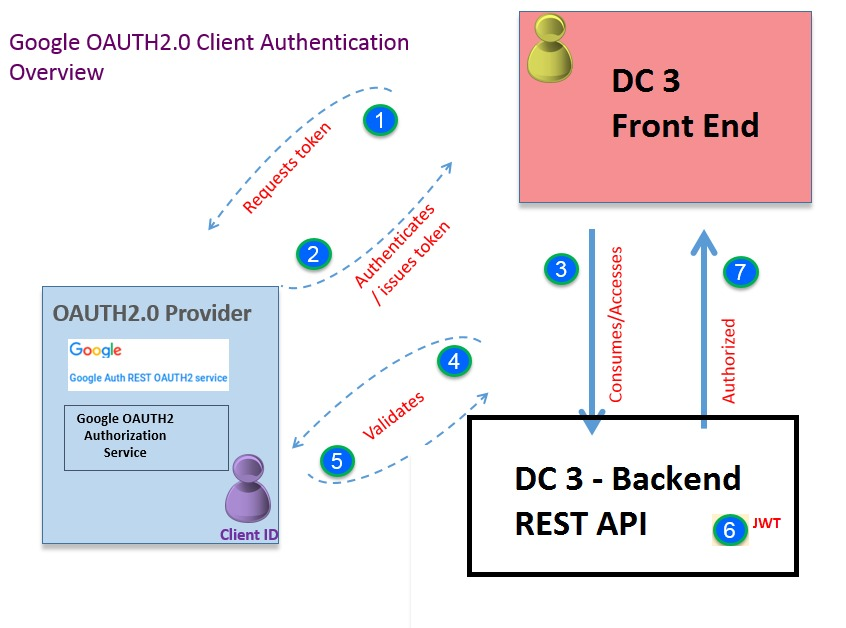
\includegraphics[width=0.5\textwidth]{images/GoogleAuth.jpeg}\\
	\caption{Authentication \& Authorization}
	\label{fig:Authentication and Authorization}
\end{figure}


\section{Database Design}
DC3 database has 8 tables. Order, Person, Order History and Order sensors are the major tables while others play an important role as well.  Designs majorly circulate around Orders table. We have normalized the database to avoid storing redundant data e.g. Order and Sensors had many to many relationship so we divided it and created another table, OrderSensors. Let’s understand the philosophy behind each table


\subsection{Company}
The company table is persisting the information about all the companies. It stores the company name and a brief description of the company. 

\begin{table}[!ht]
	%\small
	\centering
	\begin{tabular}{ |l|l|l| }
		\hline
		Id & Int - auto increment & Unique company ID \\
		\hline
		Name & varchar & Company Name \\
		\hline
		Description & varchar & Brief company description \\
		\hline
	\end{tabular}
	\caption{Company table}
\end{table}



\subsection{Address}
Address table is maintaining all kind of address across the whole system, be it order adree or customer home address. Hence it has relationship with Order and Person. Order table has two address Ids, each for pick and delivery address of the order



\begin{table}[!ht]
	%\small
	\centering
	\begin{tabular}{ |l|l|l| }
		\hline
		AddressId  & Int - Autoincrement & \\
		\hline
		StreetAddress  & varchar & \\
		\hline
		City  & varchar &\\
		\hline
		Country  & varchar &\\
		\hline
		PostCode  & int &\\
		\hline
	\end{tabular}
	\caption{Address table}
\end{table}



\subsection{Sensor}
The sensor table is a repository of unique sensors we have available in the system. It will store the names, and different possible thresholds a specific sensors has. It was designed in a generic way to store the different sensors in the same table. 




\begin{table}[!ht]
	\small
	\centering
	\begin{tabular}{ |l|l|l| }
		\hline
		Id  & Int - Autoincrement  & \\
		\hline
		Name  & varchar & \\
		\hline
		MinValue & varchar & Minimum possible reading for the sensor  \\
		\hline
		MaxValue & varchar & Maximum possible reading for the sensor\\
		\hline
		DisplayUnit  & varchar & \\
		\hline
	\end{tabular}
	\caption{Sensor table}
\end{table}


\subsection{Person}
The Person table is storing various kinds of user information. It stores personal information for the company, customer and postman. Additionally, it maintains the social login values for the user. Once a user signs up, it defaults to a customer but admin or company user can change his role to postman or admin (company) user. 

\begin{table}[!ht]
    \begin{center}
    \begin{tabular}{ |l|l|l| } 
    \hline
    Id & Int - auto increment & Unique company ID \\
    \hline
    FullName & varchar & \\
    \hline
    Email  & varchar & \\
     \hline
    Password & varchar & Minimum possible reading for the sensor \\
     \hline
    DateOfBirth & varchar & Maximum possible reading for the sensor \\
     \hline
    PersonType & varchar & Person type e.g. customer, postman or company \\
    \hline
    PersonRole & int & Stores person role or associated company id \\
    \hline
    GoogleProviderId & varchar & Google user-id \\
    \hline
    GoogleAccessToken & varchar & Logged-in user access token\\
    \hline
    \end{tabular}
    \end{center}
    \caption{Person table}
\end{table}



\subsection{Orders}
Orders table is keeping most of the data in the database and it will have a higher churn rate than any other table in the whole system. It stores a lot of referential ids from other tables than actual data e.g. pick \& drop address, person, company. 

\begin{table}[!ht]
\begin{center}
\begin{tabular}{ |l|l|l| } 
 \hline
Id & Int - auto increment & Unique Order ID \\
 \hline

OrderID & Int - AutoIncrement  & \\
\hline
PickAddressID & Int & Pick up address id\\
\hline
DropAddresID  & Int  & Drop address Id\\
\hline
PickDate  & date & Registration or pick up date\\
\hline
ArrivalDate & date & Delivery date\\
\hline
PersonID & int & Package Sender id\\
\hline
ReceiverPersonID & int & Package Receiver id\\
\hline
Status & varchar & E.g. Registered, In-Transit or Delivered\\
\hline
CompanyId & int & Reference for associated company\\

 \hline
\end{tabular}
\end{center}
    \caption{Orders table}
\end{table}

\subsection{OrderSensors}
\begin{table}[!ht]
\begin{center}
\begin{tabular}{ |l|l|l| } 
 \hline
Id & Int - auto increment & Unique company ID \\
 \hline
Name & varchar & Company Name \\
 \hline
Description & varchar & Brief company description \\
 \hline
\end{tabular}
\end{center}
    \caption{OrderSensors table}
\end{table}

\subsection{Incident}
\begin{table}[!ht]
\begin{center}
\begin{tabular}{ |l|l|l| } 
 \hline
Id & Int - auto increment & Unique company ID \\
 \hline
Name & varchar & Company Name \\
 \hline
Description & varchar & Brief company description \\
 \hline
\end{tabular}
\end{center}
    \caption{Incident table}
\end{table}

\subsection{Database Diagram}
\begin{figure}[!ht]
	\centering
	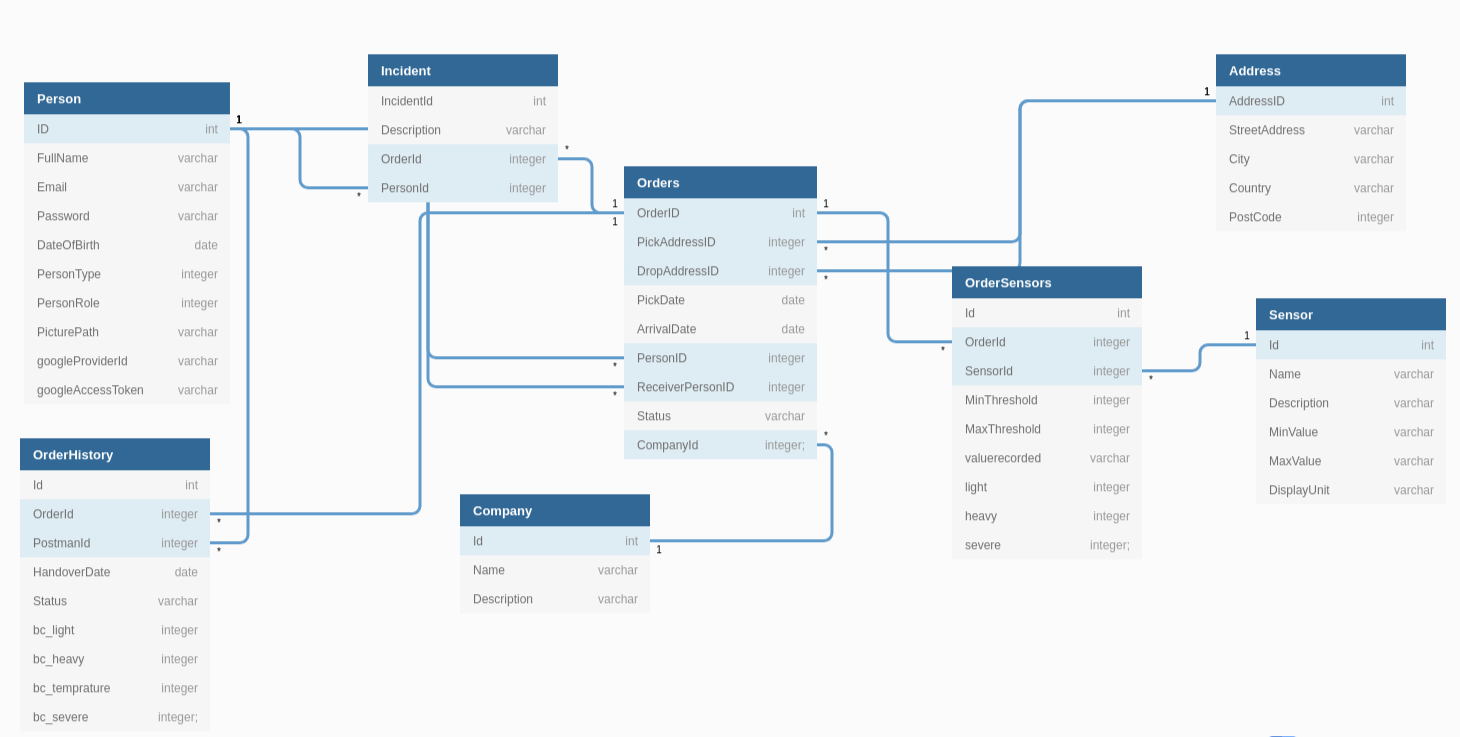
\includegraphics[width=1\textwidth]{images/IOSLDBDiagramlatex.png}\\
	\caption{Database Diagram}
	\label{fig:Database Diagram}
\end{figure}

\chapter{Implementation}
\label{cha:implementation}

\section{Costumer}
The costumer role refer to any individual who send a package through the system.
as discussed in the design paragraph the costumer has the following features:

\begin{description}[font=$\bullet$~\normalfont\scshape\color{red!50!black}]
\item register a package
\item delete a package with status "registered"
\item show a package detail view 
\item time line
\end{description}

\subsection{Register a package}
The register package process divided by two component:
\begin{description}[font=$\bullet$~\normalfont\scshape\color{red!50!black}]
\item RegisterPackage.js - view (child)
\item UserSpace.js - controller (father)
\end{description}


\begin{figure}[!ht]
	\centering
	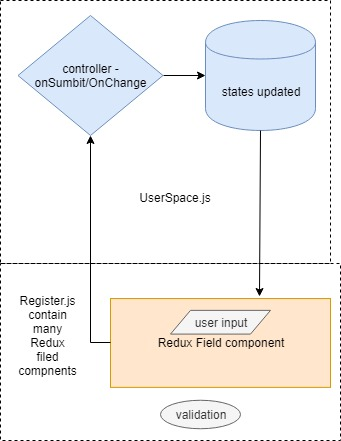
\includegraphics[width=0.5\textwidth]{images/register.jpg}
	\caption{register package process, component diagram}
	\label{fig:}
\end{figure}


The component ResgiterPackage is an assembly of Redux <Field> component.
for each input field the user enter the form get render and the state is updated
The form contain the following validation:
\begin{description}[font=$\bullet$~\normalfont\scshape\color{red!50!black}]
\item no text input filed can be left empty 
\item receiver mail must be a register user
\end{description}
i.e with out full filling the constrains the user can not press the submit button


\chapter{Evaluation}
\label{cha:evaluation}

The evaluation of the thesis should be described in this chapter
\chapter{Conclusion}
\label{cha:conclusion}

In the beginning we were given a brief idea about the project explaining that it is a dashboard for monitoring logistics data. As per the requirements it was clear that the web application is supposed to be used by three different user groups. Hence the primary focus was on the look and feel of the landing screen, navigation pane and dashboard components. Development in this part involved plenty of hit and trials; adding and removing components; re-designing old components, changing and adjusting size and placement of components on the dashboard therefore making sure that each user group has a different view of the dashboard. Using reach JavaScript makes it very convenient to embrace the hit and trial approach of work because we are able to view the changes immediately into the running local server, once the code changes are saved in VS Code. The presence of NavBar component provides a rigid classification of different components; for example Register.js is kept under Package Management category and Incident.js is kept under Incident Management category. This ensures the whole webpage does not get refreshed while navigating from one functional component to another. Considering the diversity among our team members in knowledge background and areas of expertise, it was not an easy job to immediately start working on the project development. We needed few weeks to introduce ourselves to React JS and once we started developing the web pages, we learned a lot about this technology while fiddling with the individual functionalities of every component. This knowledge and experience we have gained while developing DC3 dashboard is very priceless and some of us even look forward to pursue this track of full stack development with React/Node JavaScript and make it an integral part of our careers in Information Technology sector. We have also come across several challenges during the development phase that we have overcome with teamwork, brainstorming, collective research and individual hardwork. It was a brilliant experience to work as a team with these incredibly skilled members especially Mohammed Haseeb Asif, who single-handedly overlooked the entire development phase serving as a highly capable Project Manager with his years of impeccable experience on Software Industry.


%--------------------------------------------------------------
% TABLES, FIGURES, BIBLOGRAPHY AND APPENDICES
%--------------------------------------------------------------
\backmatter

% Lists of tables and figures
\listoftables
\listoffigures

% Bibliography
\setwidesite{}						% Set page to be wider for bibliography
\markboth{Bibliography}{bibliography}
\label{cha:bibliography}
\bibliographystyle{IEEEtran}
\bibliography{bibliography.bib}

% Use following to separate online (websites) and offline (books, papers) sources
%\printbibliography[heading=offline,filter=offline]
%\printbibliography[heading=online,filter=online]

\begin{appendices}
	\chapter{Appendix 1}
\label{appendix:listing1}

\begin{figure}[htp]
    \centering
    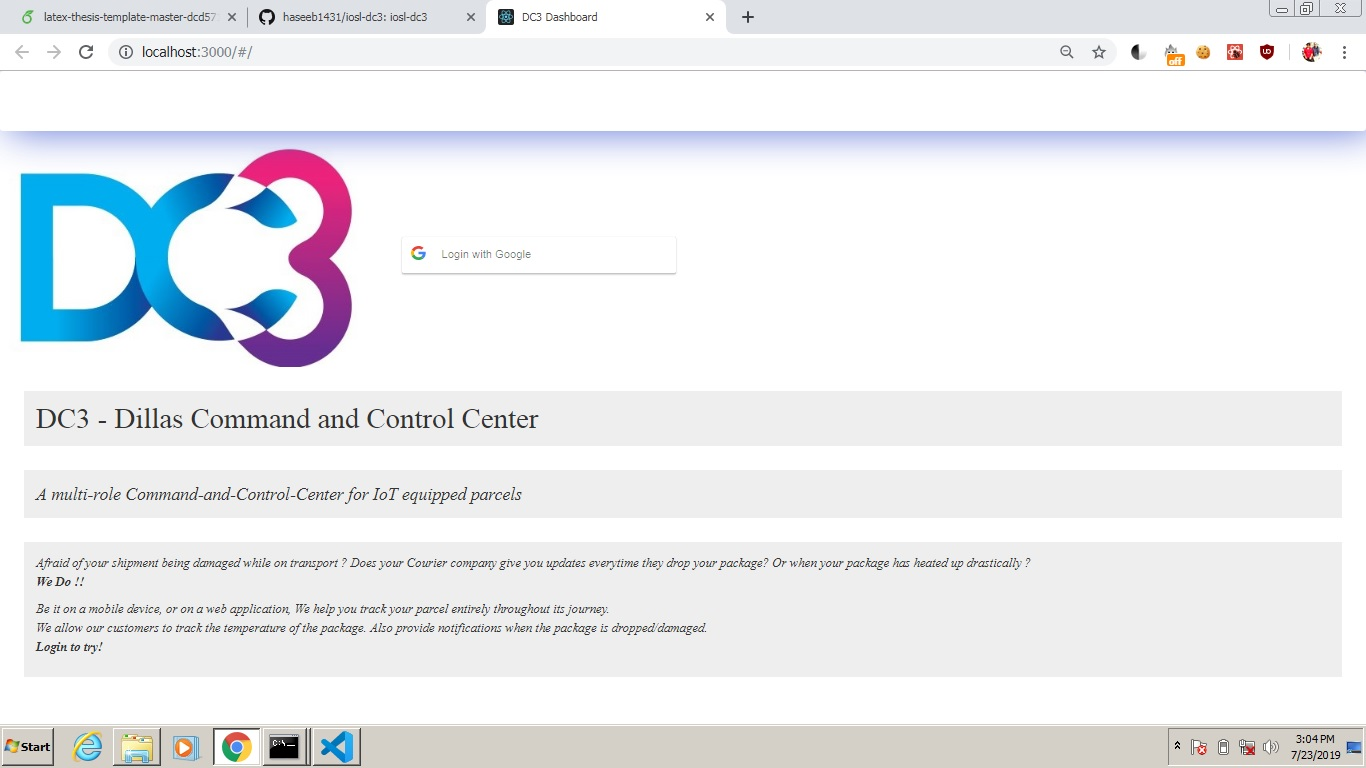
\includegraphics[width=6cm]{images/screenshots/Home.jpg}
    \caption{DC3 Landing Page}
    \label{fig:}
\end{figure}

\begin{figure}[htp]
    \centering
    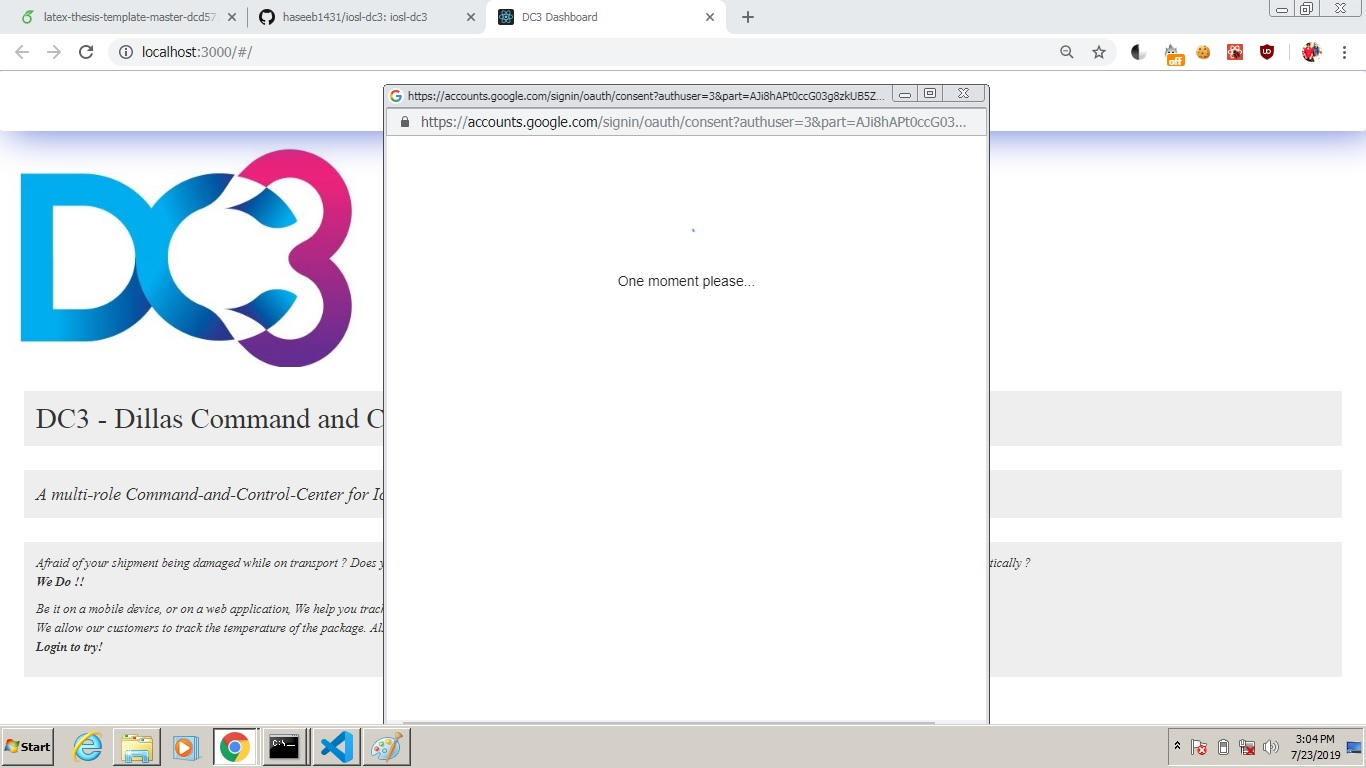
\includegraphics[width=6cm]{images/screenshots/Login.jpg}
    \caption{DC3 Login}
    \label{fig:}
\end{figure}

\begin{figure}[htp]
    \centering
    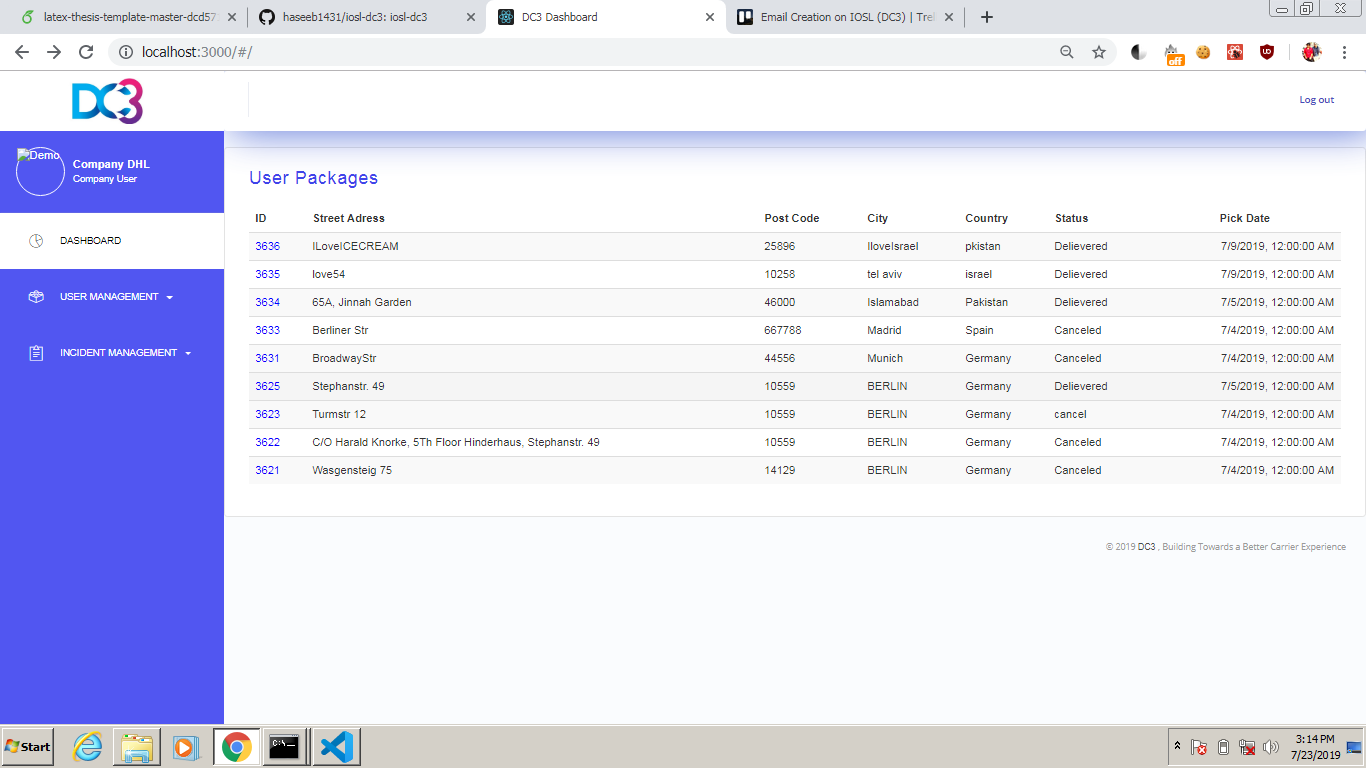
\includegraphics[width=6cm]{images/screenshots/Company_Dashboard.png}
    \caption{DC3 Company Dashboard}
    \label{fig:}
\end{figure}

\begin{figure}[htp]
    \centering
    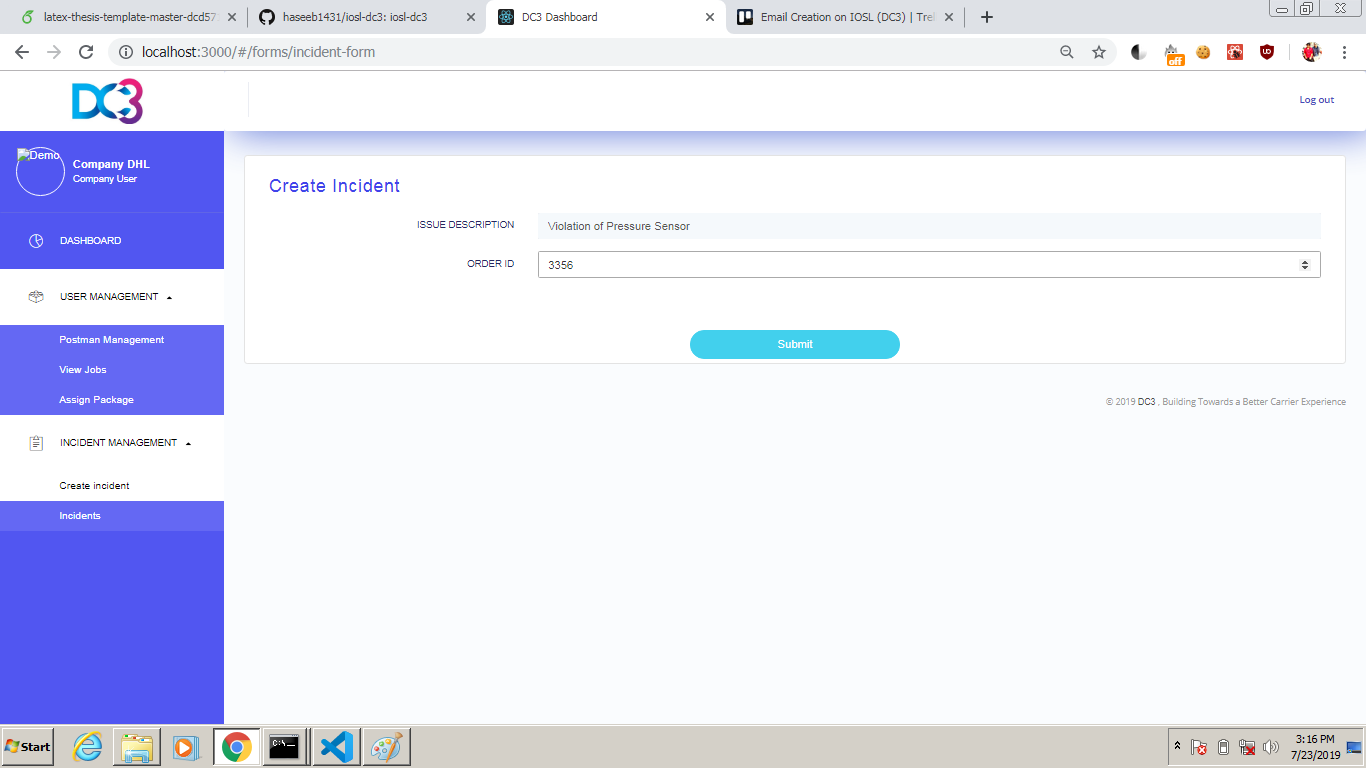
\includegraphics[width=6cm]{images/screenshots/Company_Raise_Incident.png}
    \caption{DC3 Company Raise Incident}
    \label{fig:}
\end{figure}

\begin{figure}[htp]
    \centering
    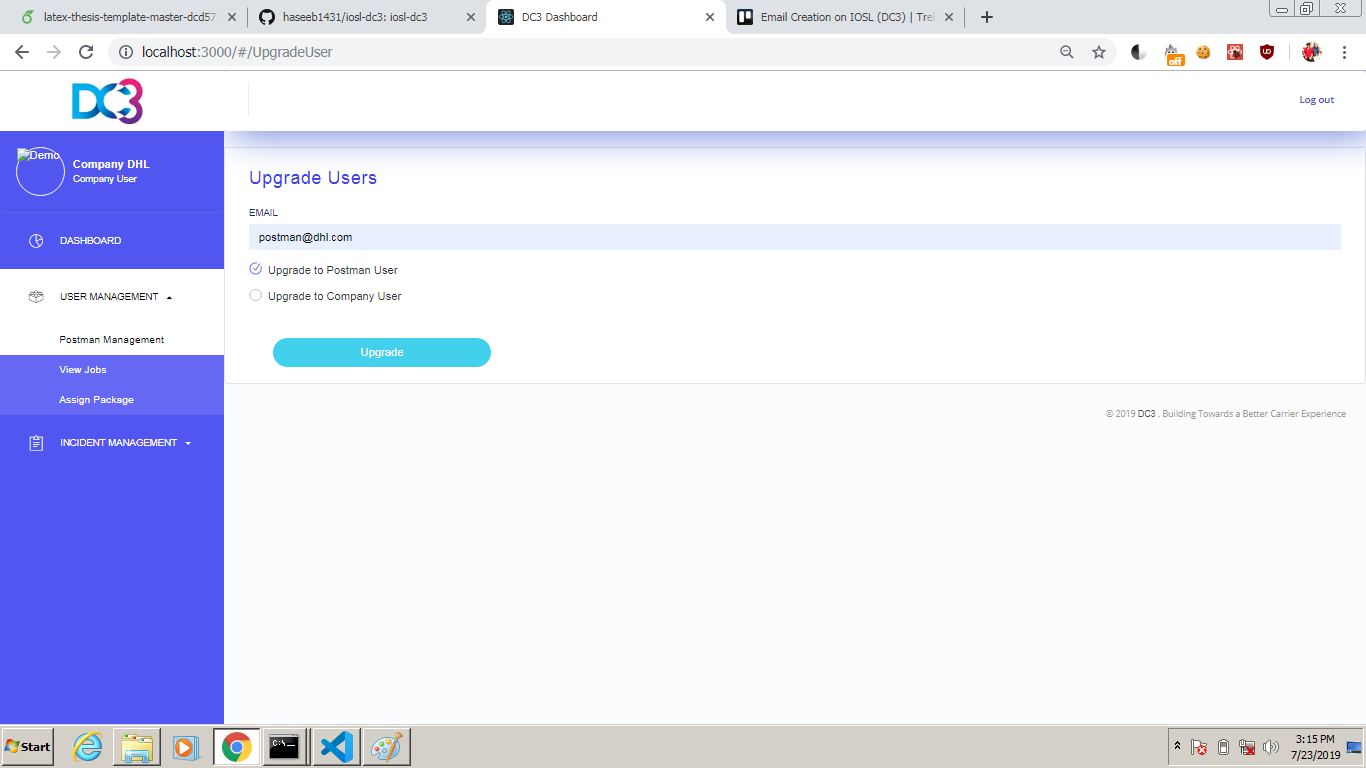
\includegraphics[width=6cm]{images/screenshots/Company_User_Mgmt.png}    \caption{DC3 Company User Management}
    \label{fig:}
\end{figure}

\begin{figure}[htp]
    \centering
    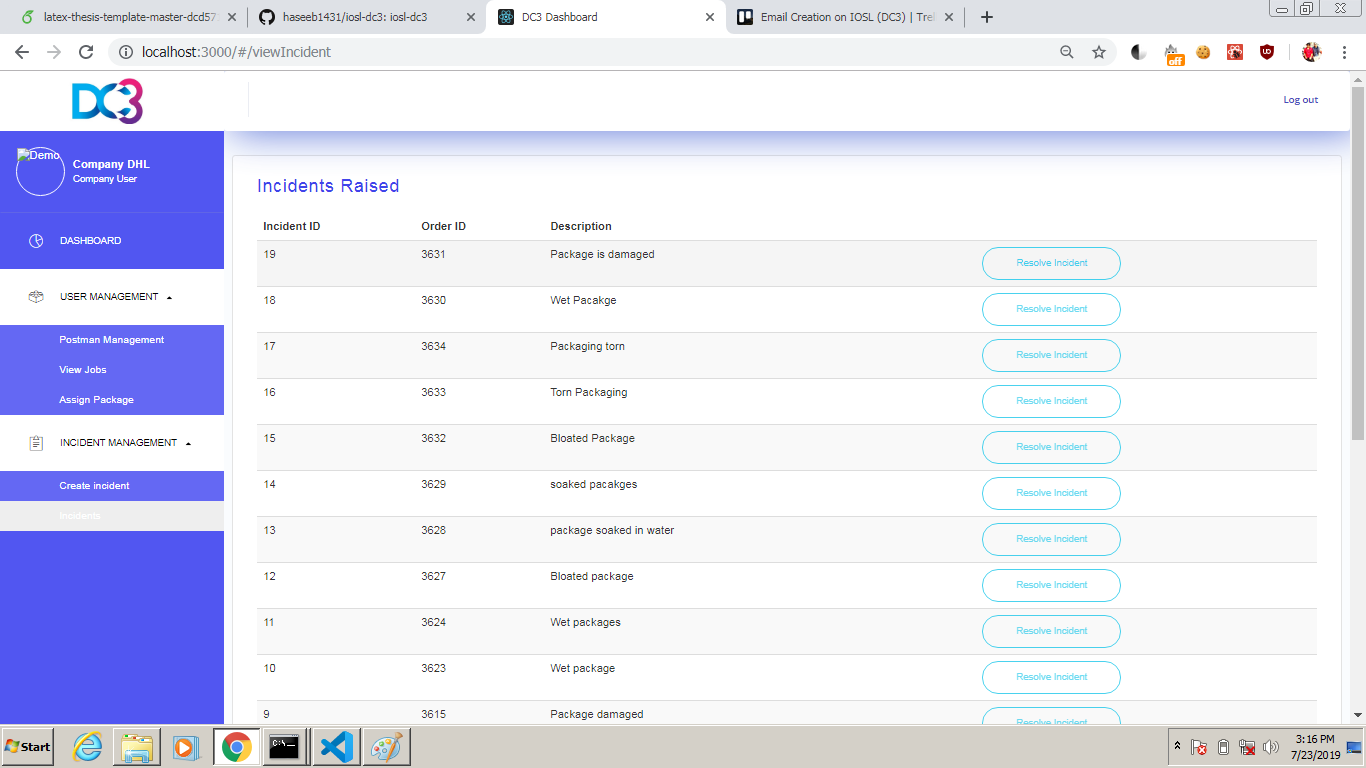
\includegraphics[width=6cm]{images/screenshots/Company_View_Incidents.png}
    \caption{DC3 Company View Incidents}
    \label{fig:}
\end{figure}

\begin{figure}[htp]
    \centering
    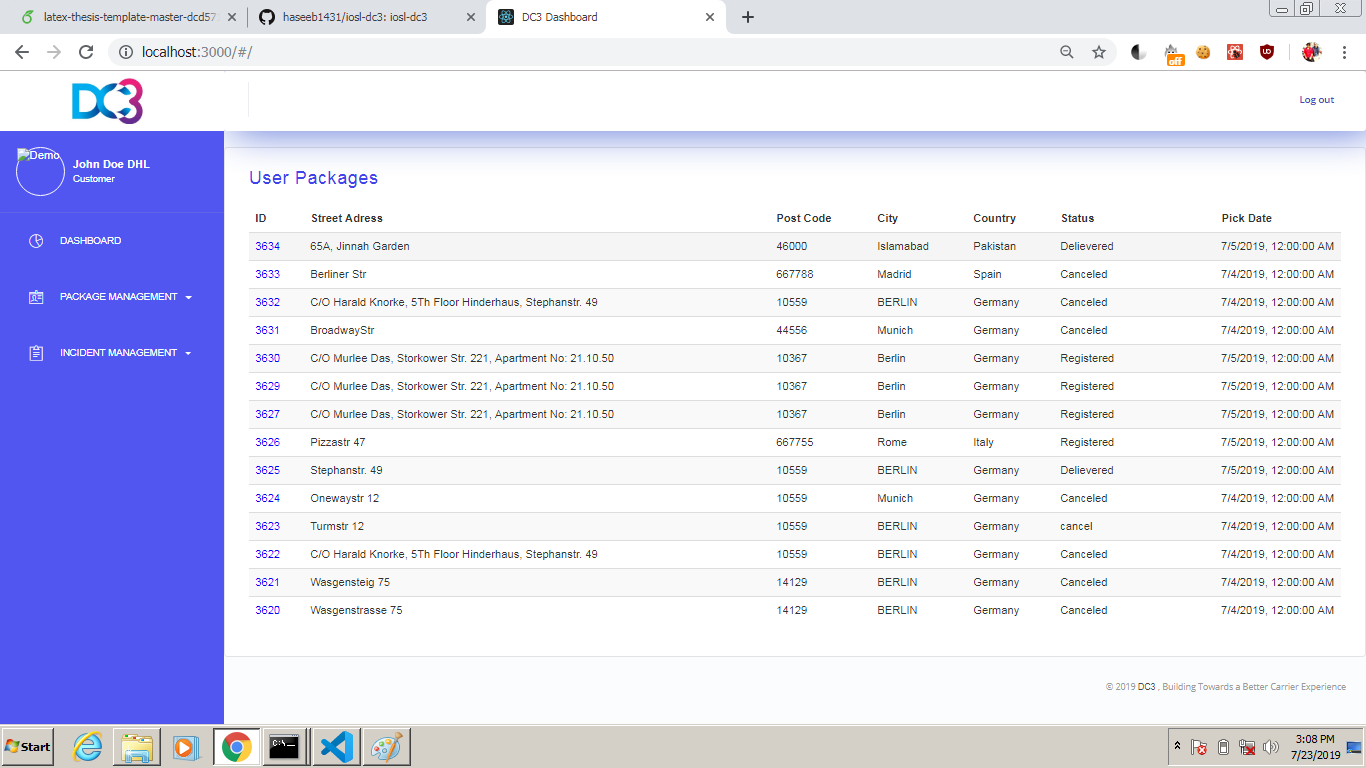
\includegraphics[width=6cm]{images/screenshots/Customer_Dashboard.png}
    \caption{DC3 Customer Dashboard}
    \label{fig:}
\end{figure}

\begin{figure}[htp]
    \centering
    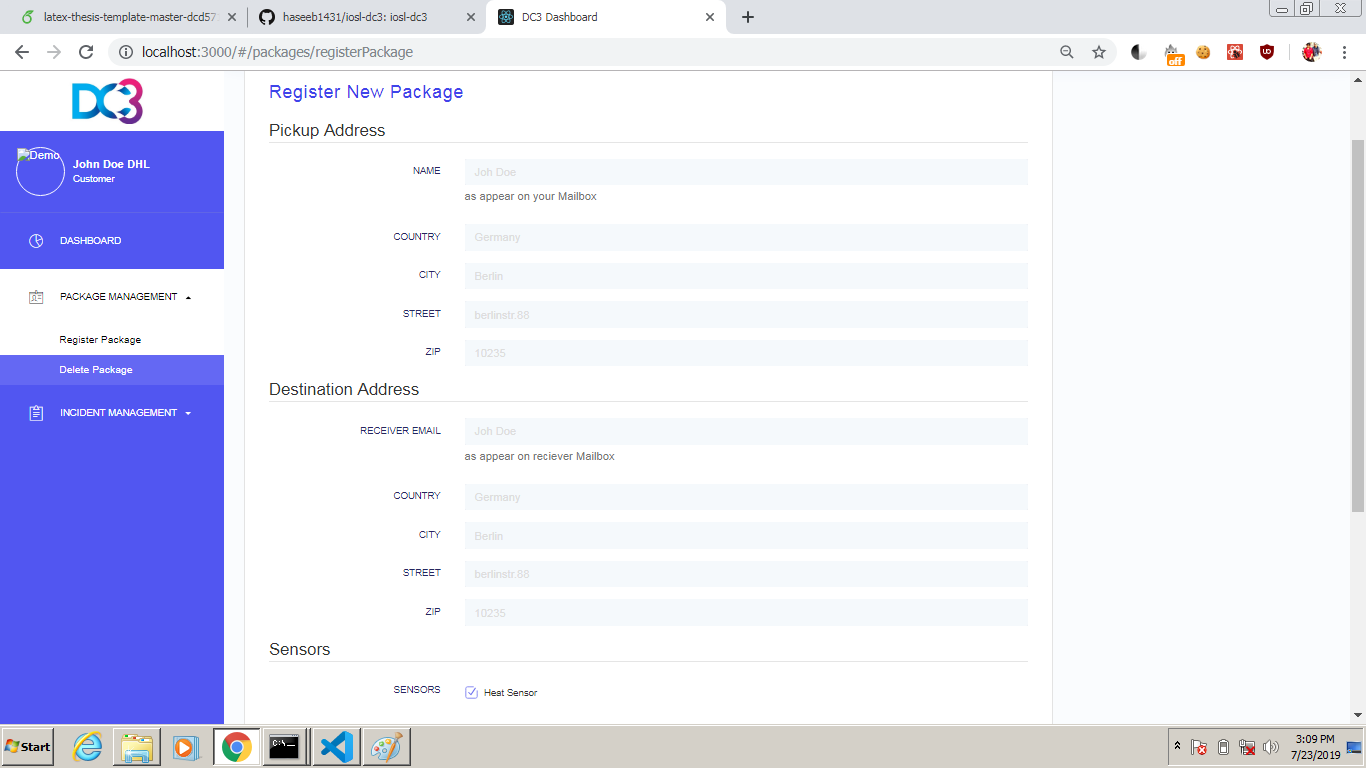
\includegraphics[width=6cm]{images/screenshots/Customer_Register_Package.png}
    \caption{DC3 Customer Register Package}
    \label{fig:}
\end{figure}

\begin{figure}[htp]
    \centering
    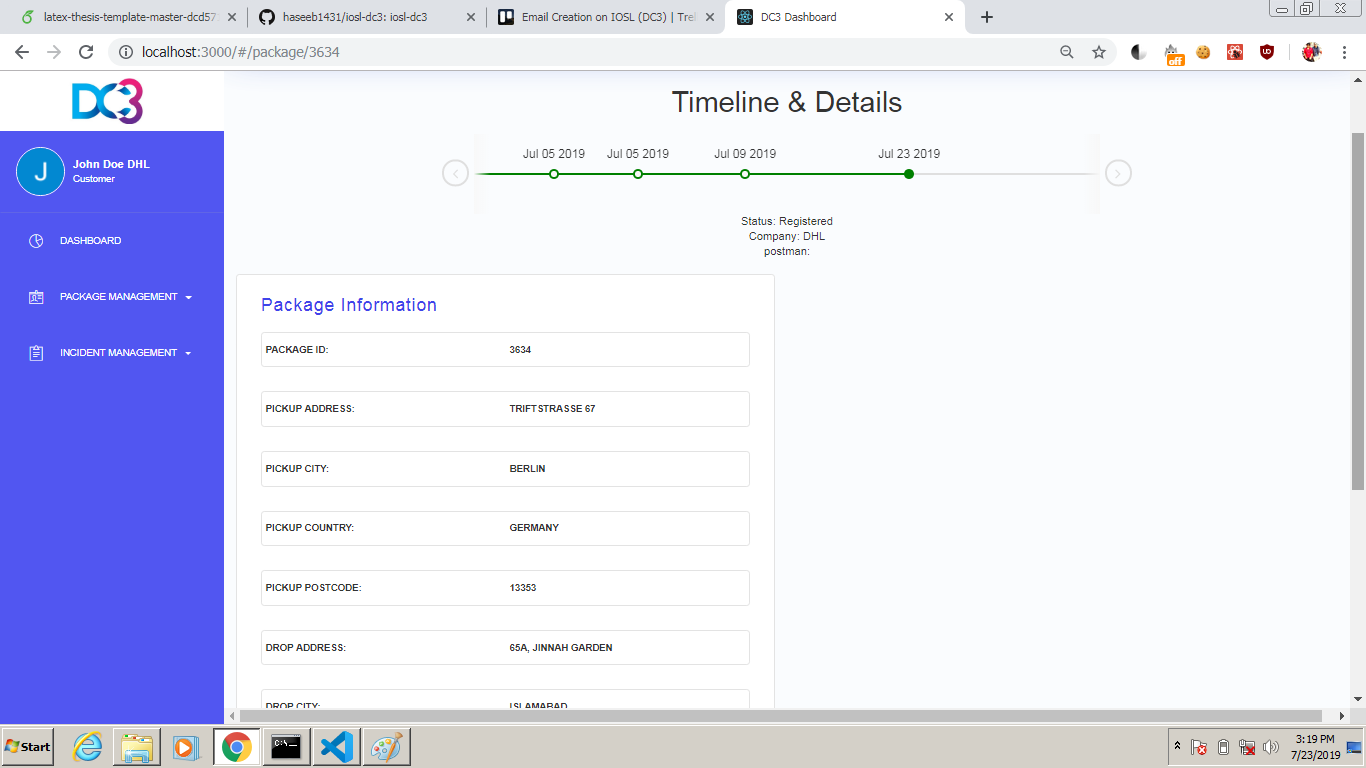
\includegraphics[width=6cm]{images/screenshots/Customer_Package_Details.png}
    \caption{DC3 Customer Package Details}
    \label{fig:}
\end{figure}


\begin{figure}[htp]
    \centering
    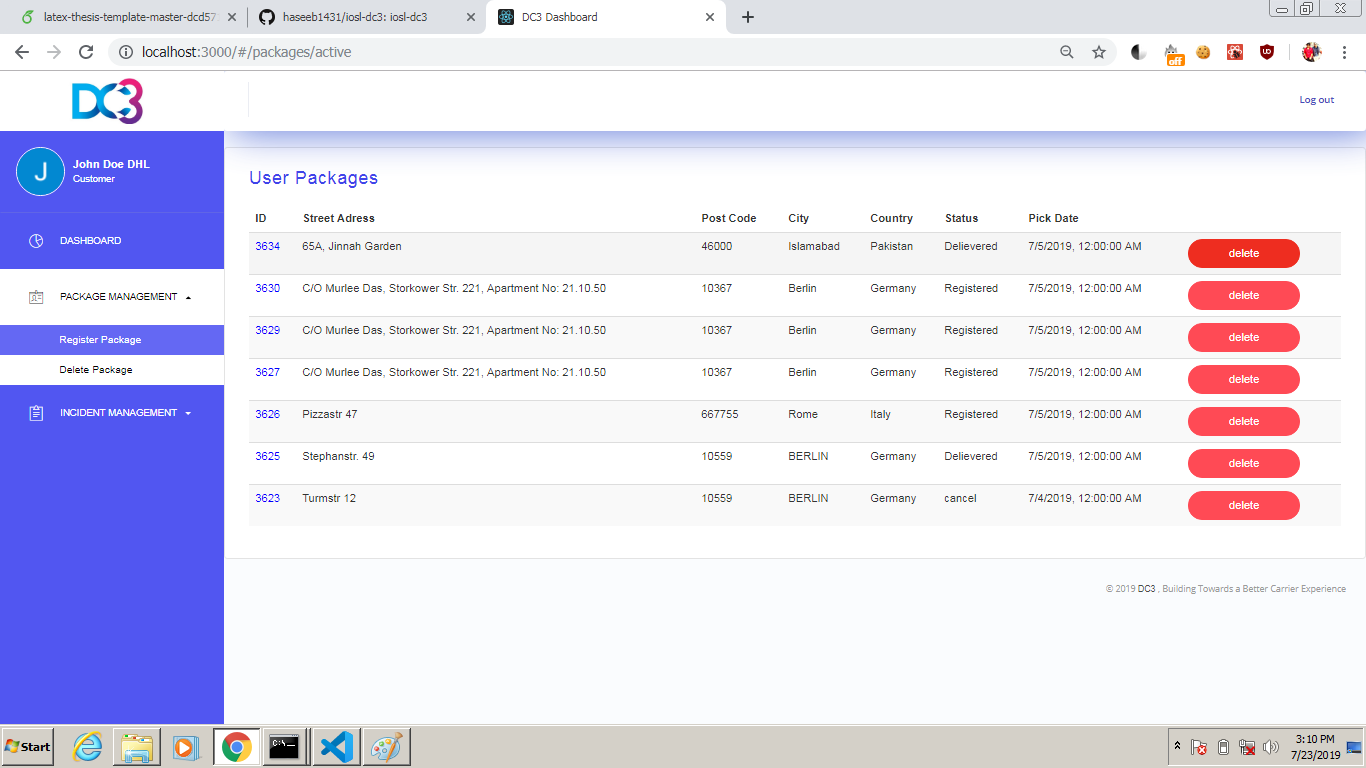
\includegraphics[width=6cm]{images/screenshots/Customer_Delete_Package.png}
    \caption{DC3 Customer Delete Package}
    \label{fig:}
\end{figure}

\begin{figure}[htp]
    \centering
    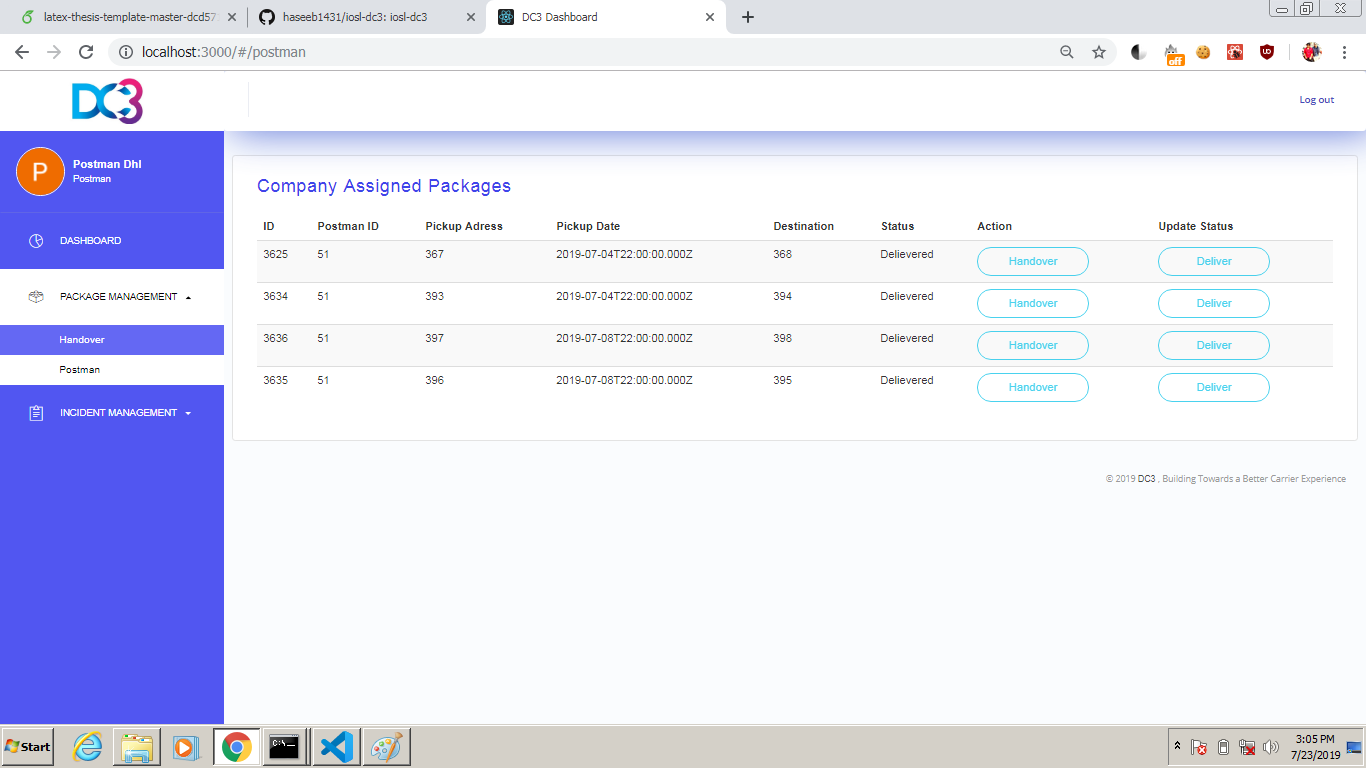
\includegraphics[width=6cm]{images/screenshots/Postman_Dashboard.png}
    \caption{DC3 Customer Postman Dashboard}
    \label{fig:}
\end{figure}

\begin{figure}[htp]
    \centering
    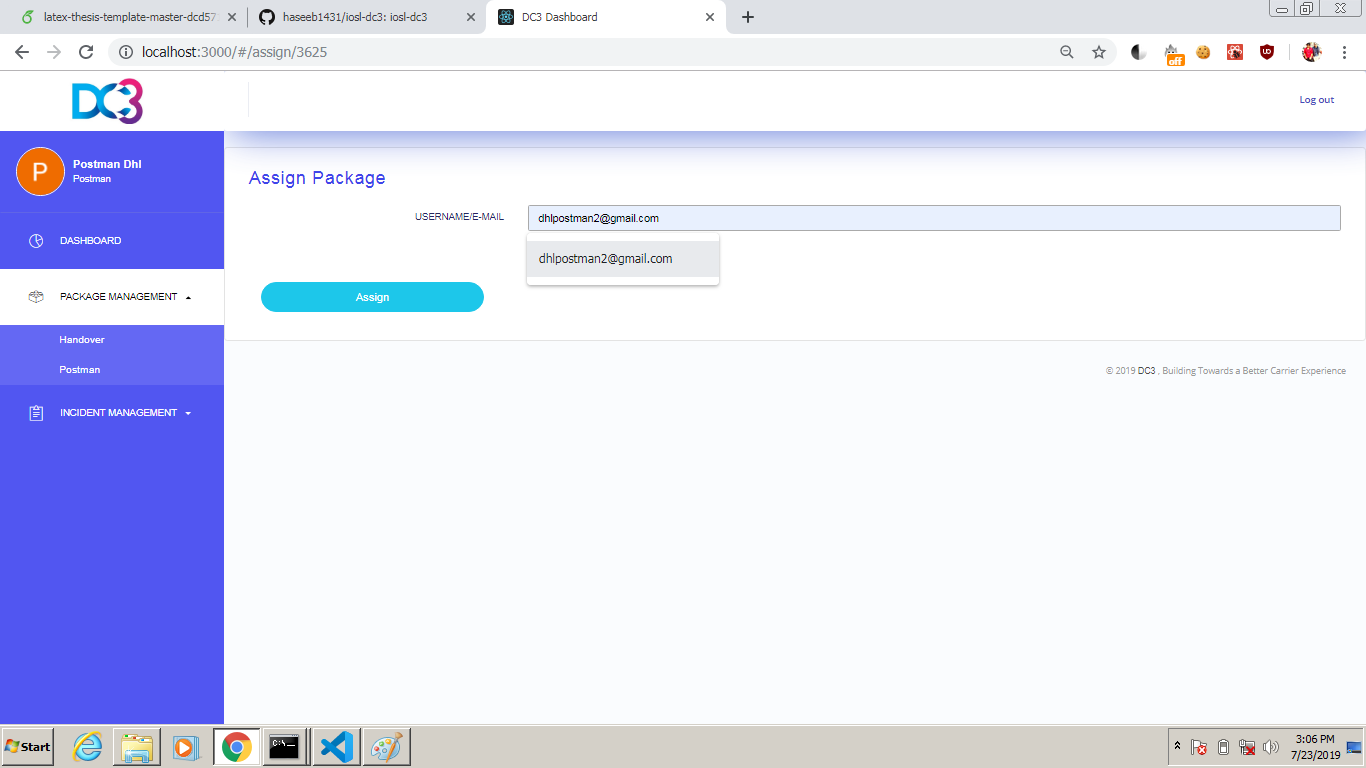
\includegraphics[width=4cm]{images/screenshots/Postman_Handover.png}
    \caption{DC3 Customer Postman Handover Package}
    \label{fig:}
\end{figure}

\begin{figure}[htp]
    \centering
    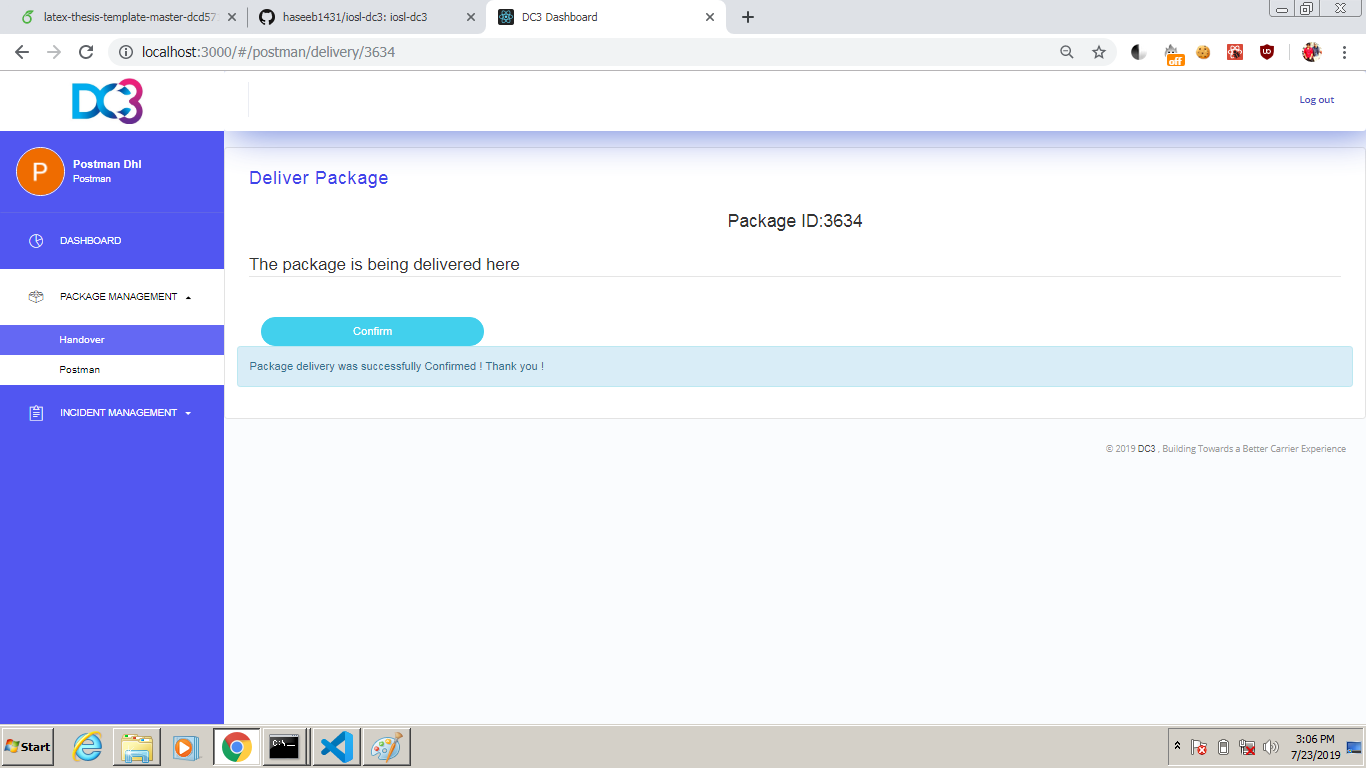
\includegraphics[width=4cm]{images/screenshots/Postman_Delivery.png}
    \caption{DC3 Customer Postman Deliver Package}
    \label{fig:}
\end{figure}


	% \input{content/99_appendices/a02_listings}
	% \input{content/99_appendices/a03_listings}
\end{appendices}

\end{document}
